\documentclass[bsc]{abdnthesis}

%% For citations, I would recommend natbib for its
%% flexibility, particularly when named citation styles are used, but
%% it also has useful features for plain and those of that ilk.
%% The natbib package gives you the following definitons
%% that extend the simple \cite:
%   \citet{key} ==>>                Jones et al. (1990)
%   \citet*{key} ==>>               Jones, Baker, and Smith (1990)
%   \citep{key} ==>>                (Jones et al., 1990)
%   \citep*{key} ==>>               (Jones, Baker, and Smith, 1990)
%   \citep[chap. 2]{key} ==>>       (Jones et al., 1990, chap. 2)
%   \citep[e.g.][]{key} ==>>        (e.g. Jones et al., 1990)
%   \citep[e.g.][p. 32]{key} ==>>   (e.g. Jones et al., p. 32)
%   \citeauthor{key} ==>>           Jones et al.
%   \citeauthor*{key} ==>>          Jones, Baker, and Smith
%   \citeyear{key} ==>>             1990

% \usepackage[round,colon,authoryear]{natbib}
% \setlength{\bibsep}{0pt}
% \bibliographystyle{apalike}

\usepackage[T1]{fontenc}
\usepackage{hyperref}
\usepackage{amsmath,amsthm}
\usepackage{color} 
\usepackage{graphicx}
\usepackage{float}
\usepackage{algorithm2e}
\usepackage{tikz}
\usepackage{array}
\usepackage{setspace}
\usetikzlibrary{decorations.pathmorphing}
\usetikzlibrary{decorations.fractals}
\usepackage{mdwlist}
\usepackage{fancyvrb}
\DefineVerbatimEnvironment{code}{Verbatim}{fontsize=\small}
\DefineVerbatimEnvironment{example}{Verbatim}{fontsize=\small}
\newcommand{\ignore}[1]{}

\newtheorem*{defn}{Definition}
\newtheorem*{thm}{Theorem}
\newtheorem*{exa}{Example}
\newtheorem*{no}{Note}

\graphicspath{ {./Figures/} }

\title{Particle Swarm Optimisation \\ to solve the Portfolio Selection Problem \\ in a Function Based Environment \\ (30 Credit Course)}
\author{Anthony Sergio Chapman}
\Supervisor{Dr. Wei Pang}
% IMO this is a bit silly, but some like to include these. To remove,
% delete this declaration and remove the option from the
% \documentclass definition above.
%\qualifications{PhD, Computer Science, University College London, 1997\\%            
%BEng (Hons.) Electrical and Electronic Engineering, The University of Wales, Swansea, 1992}
\school{Department of Computing Science}

%%%% In the final submission of a thesis, this should only be the year
%%%% of submission.  However, it is useful to use \date{\today} for drafts so that
%%%% they don't get mixed up.
    
\date{2014}

%% It is useful to split the document up as chapters and include
%% them.  LaTeX will sort out all the numbering and cross-referencing
%% for you --- if you run it enough times!

%% If you want to include only a couple of chapters then use the
%% \includeonly{} command with a list of the file/chapter names that
%% you wish to include.  NB, this must be in the preamble.

% \includeonly{introduction,faq,chap1}

\def\sfthing#1#2{\def#1{\mbox{{\small\normalfont\sffamily #2}}}}

\sfthing{\PP}{P}
\sfthing{\FF}{F}

%% This will make sure that all cross-references are correct (including
%% references to those file not included) but will produce a dvi
%% file with only those files/chapters you specify included.

\begin{document}

%%%% Create the title page and standard declaration.

\maketitle
\makedeclaration

%%%% Then the abstract and acknowledgements

\begin{abstract}
  This research project aims to investigate how the Particle Swarm Optimisation (PSO) algorithm could be applied for multi-dimensional optimisation in a real-world domain, namely finding an optimal portfolio to invest in, given a set of assets and their expected returns. The Particle Swarm Optimisation algorithm, created by James Kennedy and Russell Eberhart, belongs to the field of Swarm Intelligence. It uses a collection of particles (a swarm) to explore a given search space for an optimal value. To be able to solve the portfolio optimisation problem, a way to measure and compare different portfolio had to be created. Using two-sided coherent risk measure, created by Zhiping Chen and Yi Wang, and concepts from mathematics, measure theory, the portfolio optimisation problem turned into a function what the PSO algorithm is able to optimise. 

  The main goal of this project is to create a reliable method for computing and comparing a portfolio's success or failure in order for the algorithm to be able to find an optimal one. Secondary goals such as experimenting and expanding the PSO algorithm were also achieved. Finally, the effectiveness of the resulting approach was assessed through experimentation and different parameter settings. The report shows the background research, design, implementation, testing and experimentation with the expanded Deterministic Dendritic Cell Algorithm based on datasets from two different domains (Port Scanning data and SEPA River data). 
\end{abstract}

\begin{acknowledgements}
  Firstly, I would like to thank my supervisors, Dr. Wei Pang, for providing help and support throughout the whole project. His advice, enthusiasm and knowledge of the field have always pointed me in the right direction with the research. 

  Secondly, I would also like to thank Dr. Fernando Rubio, from U.C.M., for proving additional support for expanding the Haskell PSO implementation and finding time to answer my inquiries. 

  Lastly, thanks to all my 205 buddies for providing moral support and advise at all hours of the day.
\end{acknowledgements}

%%%% It should have a table of contents, but delete the other two as
%%%% necessary.

\tableofcontents
\listoftables
\listoffigures

\chapter{Introduction\label{chap:intro}}
This section provides an overview of the project and explains the basic principles of the initial approach and ideas for expansion. It contains a list of primary and secondary goals as well as motivation for carrying out this research.

  \section{Overview} % (fold)
  \label{sec:overview}
  Swarm Algorithms that belong to the Swarm Intelligence Systems were inspired by the behaviour of ant colonies, bird flocking, animal herding, bacterial growth, and fish schooling. As flocks of birds, the artificial swarm is able find an optimal location through communication with local agents as well as the environment. Swarm Algorithms have proven to be effective in providing ways to find global optima in potentially troublesome search spaces. The techniques used in Swarm Intelligence Systems closely related to artificial intelligence and are often applied to simulations, robotics and optimisation problems. 

  The Particle Swarm Optimisation algorithm belongs to the field of Swarm Intelligence Systems and optimizes a problem by having a population of candidate solutions, called particles, moving these particles around in the search-space according to simple mathematical formula over the particle's position and velocity, shown in Equation~(\ref{eq:pso}). Each particle's movement is influenced by its local best known position but, is also guided toward the best known positions in the search-space, which are updated as better positions are found by other particles. Originally, PSO was designed to simulate bird flocking behaviour \cite{pso}, it was later discovered that it would be used to find optimal positions, such as a flock of pigeons finding food in a large city.

  Portfolio optimisation lies at the heard of investment banking. A novel way to measure a portfolio's risk using both upside and downside risk measure was introduced by Zhiping Chen and Yi Wang. In order to make this into something that the PSO can optimise, I took methods from measure theory to given a sense of distance or deviation when any constraint is violated. I introduced a penalty value to exaggerate this deviation and force the algorithm to boycott results from such a deviation.
  % section overview (end)

  \section{Motivation} % (fold)
  \label{sec:motivation}
  Over the past twenty years the amounts of data that is being produced by the financial market have increased drastically, it is essential to use efficient algorithms to analyse such data. The Particle Swarm Optimisation algorithm has already been effectively used in various applications, mainly  biomedical, clustering, and modeling. However, the use of PSO to find optimal values when trading stocks or other securities has not been exploited thoroughly enough. Given that dealing with the financial market requires dealing with vasts amounts of numerical data, I believe one can formulate complex financial concepts, such as optimising a portfolio, and apply them to PSO. The PSO algorithm could potentially be applied to various systems and applications to a wide range of domains and an application to solve the portfolio selection problem could start a new generation of evolutionary financial solutions. 
  
  This idea was greatly inspired by both my supervisor, by introducing me to the world of evolutionary algorithms, and recently discovered ways to measure a portfolio's risk \cite{two_sided_risk}. The author provides a comprehensive overview of portfolio risk measurement, describing how it can be used to optimise a portfolio as well.
  % section motivation (end)

  \section{Primary Goals} % (fold)
  \label{sec:primary_goals}
  A list of primary goals which need to be completed in order to classify the research project as a success.
  \begin{itemize}
    \item Understand the principles behind Particle Swarm optimisation.
    \item Design an appropriate expansion to solve the portfolio selection problem.
    \item Understand the principles begin portfolio risk measure.
    \item Test the resulting application and assess whether it can be used in a professional environment.
  \end{itemize}
  % section primary_goals (end)

  \section{Secondary Goals} % (fold)
  \label{sec:secondary_goals}
  Secondary goals could be added to the project depending on time-constraints and success of completing the primary goals.
  \begin{itemize}
    \item Compare my implementation to that of an investment manages. 
    \item Write a simple GUI for the application.
  \end{itemize}

\chapter{Background}\label{chap:background}
  In order to expand and adapt existing Particles Swarm Optimisation methods an initial background research has to be done to fully understand the concepts involved. Similarly to apply the algorithm to solve the portfolio optimisation problem, a deep understanding on how to formulate the problem in a way that the algorithm will understand will have to be made. 

  This chapter describes the key concepts which I will use and eventually expand, implement and improve. Section~\ref{sec:particle_swarm_optimisation} provides the ideas and methods for PSO. Section~\ref{sec:portfolio_management} gives some background on how to use two-sided coherent risk measure\cite{two_sided_risk} to solve the portfolio selection problem. Section~\ref{sec:haskell} describes some of Haskell's attractions. 

  % I plan to gain such knowledge by a mixture of methods including: past lecture slides, power-point presentations, research papers, online teaching videos and visiting the library as well as other ways.

  \section{Particle Swarm Optimisation} % (fold)
  \label{sec:particle_swarm_optimisation}
    % Particle Swarm Optimisation (PSO) \cite{pso,pso2,pso3,pso4} is a metaheuristic inspired on the social behaviour of flocks of birds when flying and on the movement of shoals of fish. A population of entities moves in the search space during the execution on the algorithm. These entities perform local interactions (with other particles as well as the environment).

    % Assuming worker bees are searching for a patch of flowers with the most pollen, also assume that the bees

  Particle swarm optimization (PSO) is a population based  stochastic optimization technique developed by Kennedy and  Eberhart in 1995, discovered through simplified social model simulation \cite{pso,pso2,pso3,pso4}. It simulates the behaviour of bird flocking involving the scenario of a collection of birds randomly looking for food in a search space. None of the birds know where the food is located, but they do know how far the food location is from their current positions. An effective technique for the bird to find food is to adjust their velocity according to the bird which is nearest to the food. PSO was motivated from this scenario and was developed to solve complex optimization problems, where the optimum position of the fitness function is where the food is located and all the birds are the particles searching for this optimum position. 

  An interesting thought is presented in \cite{pso} is that PSO can be used to model human social behaviour. One important difference, one that I find so fascinating, is its abstraction. It states that humans adjust not only their physical movements but also our cognitive position too; ``we tend to adjust our beliefs and attitudes to conform with those of our social peers''\cite{pso}. One of the major distinctions in this model compared to that of bird flocks or school's of fish is that collision works differently; ``two individuals can hold identical attitudes and beliefs without banging together, but two birds cannot occupy the same position in space without colliding''.

  In the conventional PSO, the behaviour displays particles in a multidimensional space where each particles has two properties: a position vector and a velocity vector. Each particle $i$ in the swarm has the properties shown in (\ref{eq:PSO_stuff}):
    % \begin{itemize}
    %   \item $X_i^k$ : The current position of particle i at time k.
    %   \item $V_i^k$ : The current velocity of particle i at time k. 
    %   \item $Pbest_i^k$ : The personal best position of particle i at time k. 
    %   \item $Gbest^k$ : The global best position of particle i at time k. 
    % \end{itemize}
    \begin{equation} \label{eq:PSO_stuff}
      \begin{split}
        & V_i^t \text{ : The velocity of particle i at time t.} \\
        & X_i^t \text{ : The current position of particle i at time t.} \\
        & Pbest_i^t \text{ : The personal best position of particle i at time t.} \\
        & Gbest^t \text{ : The global best position of particle i at time t.} \\
      \end{split}
    \end{equation}
    At each step, the velocity of the $ith$ particle will be updated according to the following equation:
    \begin{equation} \label{eq:vel}
      \begin{split}
        V_{i}^{t+1} & = \omega V_{i}^{t} + c_1 r_1 \times \Big( Pbest_{i}^{t} - X_{i}^{t} \Big) + c_2 r_2 \times \Big( Gbest^{t} - X_{i}^{t} \Big) \\
        \text{where} & \\
        & V_i^{t+1} \text{ : The velocity of particle i at time t + 1.} \\
        & V_i^t \text{ : The velocity of particle i at time t.} \\
        & X_i^t \text{ : The current position of particle i at time t.} \\
        & \omega \text{ : Inertia weight parameter.} \\
        & c_1, c_2 \text{ : Acceleration coefficients.} \\
        & r_1, r_2 \text{ : Random numbers between 0 and 1.} \\
        & Pbest_i^t \text{ : The personal best position of particle i at time t.} \\
        & Gbest^t \text{ : The global best position of any particle at time t.} \\
      \end{split}
    \end{equation}
  In the updating process shown in Equation (\ref{eq:vel}) the acceleration coefficients $c_1, c_2$ ($c_1$ determines the importance one following the individual personal best whereas $c_2$ determines the importance of following the particles with the global best position)and the inertia weight $\omega$ (which states how stubborn a particle is at not deviating from their path, regardless of previous results) are predefined, and $r_1, r_2$ (these introduce the concept of randomness so that a particles is able to switch between following their personal best and that of the whole swarm) are uniformly generated random numbers in the range [0,1].

  The following algorithm \ref{eq:pso} is one of the standard PSO. The pseudo-code outlines the procedures implemented in \cite{haskellPSO}, it will be followed by an explanation on how it works.\\
  \begin{algorithm}[H] \label{eq:pso}
    \mbox{\textbf{Initialisation}} \\
    \For{i = 1,\dots,S}{
      initPosition(i) \\
      initBestLocal(i) \\
      \If{i = 1}{initBestGlobal()} 
      \If{improvedGlobal(i)}{updateGlobalBest(i)} 
      initVelocity(i)
    }
    \mbox{\textbf{Main program}} \\      
    \While{not endingCondition()}{
      \For{i - 1,\dots, S}{
        createRnd($r_1,r_2$) \\
        updateVelocity(i$,r_1,r_2$) \\
        updatePosition(i) \\
        \If{improvedLocal(i)}{updateBestLocal(i)}
        \If{improvedGlobal(i)}{updateGlobalBest(i)}
      }
    }
    \caption{PSO pseudo-code.}
  \end{algorithm}
  
  In Algorithm~\ref{eq:pso} $S$ is the number of particles in a swarm, one can see the pseudo-code for a standard PSO. A step by step explanation of Algorithm~\ref{eq:pso} is as follows: First, there is an initialisation for all the particles in the PSO, for every particle $i$, \textit{initPosition(i)} randomly created a particle with a designated position in the search space. For the first step, \textit{initBestLocal(i) = initPosition(i)}, but it will be updated afterwards. Then the $if$ function makes a first global best and if any other particles has a better global best position it will be set as the new global best. \textit{initVelocity(i)} gives particle $i$ an initial velocity which is randomly generated. 

  After the initialisation, the core of the PSO method is executed until the \textit{endingCondition()} is satisfied, which can be the number of iterations or an improvement threshold. In the body of the \textit{While} loop all particles are updated. The first step is to generate random numbers used in the velocity Equation~(\ref{eq:vel}). Then the actual velocity is updated. In the next step,\textit{updatePosition(i)} updates the position of a particles in the search space and checks the fitness function value for improvement or not. At the end of the \textit{for} loop, if \textit{improvedLocal(i) = True} then updates the local best position and finally it is similar for updating the global best position. 
  % section particle_swarm_optimisation (end)

  \section{Portfolio Optimisation} % (fold)
  \label{sec:portfolio_management}
  The term portfolio refers to a collection of investments such as stocks, bonds or other securities \cite{portfolio}. For this project we will focus on stocks but it would be trivial to include other such securities into the application as they behave in a similar manner to stocks. Portfolio Optimisation is the process of choosing the proportion of various assets to be held in a portfolio in such a way that any other choice would result in an equal or worst portfolio, here we have referred to the comparison of portfolio from the rate of return or the level of risk, ie one portfolio is better than another if it has a lower level of risk or higher rate of return. 

  This project will focus on the two-sided coherent risk measure introduced in \cite{two_sided_risk}. This revolutionises how risk can be calculated as it takes into account both downside as well as upside risk in unison. Compared to previous risk measures this new measure has the following advantages:
  \begin{itemize}
    \item The whole domain loss distribution information is utilised, making it superior for finding robust and stable investment decisions.
    \item Suitably selecting the combination coefficient and the order of the norm of the downside random loss, it is easy reflect the investor's risk attitude and to control the asymmetry and fat tails of the loss distribution.
    \item It is easy to formulate and compute, therefore easier to apply to optimisation models.
  \end{itemize}

  Now this is where some mathematical background is needed, let $\| X \|_p = (E_Q |X|^p)^{\frac{1}{p}}$, $\|X\|_\infty = ess.sup \{ |X|\}$, $\sigma_p^{\pm} (X) = \|(X-E_Q[X])^{\pm}\|_p$, as described in \cite{two_sided_risk}. As already mentioned, this two-sided risk measure takes into account both sides of the loss distribution, so relative to the expected return value $E_Q[X]$, the random variable $(X-E_Q[X])^-$ is the ``downside risk'' of $X$, which according to \cite{two_sided_risk} might be more crucial to an application than the analogues ``upside risk'' variable $(X-E_Q[X])^+$.

  This is where the name, \textit{two-sided risk measure}, comes from; it considers both sides or risk, downside and upside. Due to the way downside and upside risk can be represented and the monotonically increasing property of $\| \cdot \|_p$ with respect to p, the two-sided risk measure can be determined by the following equation:
  \begin{equation} \label{eq:two-sided}
    \begin{split}
      & \text{For } 1 \leq p \leq \infty \text{ and } a \in [0,1] \\
      \rho_{a,p}(X) & = a \sigma_1^+(X) + (1-a)\sigma_p^-(X) - E_Q[X ]\\
      & = a \|(X-E_Q[X])^+\|_1 + (1-a) \|(X-E_Q[X])^-\|_p - E_Q[X] \\
    \end{split}
  \end{equation}

  $\rho_{a,p}(X)$ in Equation~(\ref{eq:two-sided}) is generated by first taking the 1-norm of the positive deviation and the $p$-norm of the negative deviation and then taking the combination of these two norms. The inclusion of $- E_Q[X]$ in Equation~(\ref{eq:two-sided}) ensures that $\rho_{a,p}(X)$ is coherent \cite{two_sided_risk}. 

  One of the advantages proposed for two-sided coherent risk measure was that it would be easy to reflect an investor's attitude towards risk, this is achieve by the variables $p,a$ in $\rho_{a,p}(X)$ in Equation~(\ref{eq:two-sided}). An investor's risk adverse attitude is represented by $p$, where the larger $p$ is, the more risk the investor is willing to take, so small $p$ low risk, large $p$ high risk. In Equation~(\ref{eq:two-sided}) $a$ is the factor controlling the balance between good and bad volatility \cite{two_sided_risk}, $a \to 0$ represents an investors' attitude towards good volatility and $a \to 1$ would be the opposite. Thus different investors might choose different values for $p$ and $a$.

  A reader might not see how Equation~(\ref{eq:two-sided}) has much to do with optimising a portfolio from a first glance, a quick example will be shown to illustrate its use. Suppose we have $N$ assets to choose from and for $i \in [1,N]$ let $x_i \in [0,1]$ be the proportional weight of asset $i$ in the portfolio, let $r_i \in \mathbb{R}$ be a variable which represents the rate of return of asset $i$ and $\widehat{r}_i$ be the expected return of asset $i$. Then the rate of return of a portfolio can be expressed as $R = \sum_{i=1}^N x_i r_i$ and the expected return $\widehat{R} = \sum_{i=1}^N  x_i \widehat{r}_i$

  From Equation~(\ref{eq:two-sided}) we can measure the risk of a portfolio as follows:
  \begin{equation} \label{eq:portfolio-risk}
    \begin{split}
      \rho_{a,p}(R) & = a \|(R-\widehat{R})^+\|_1 + (1-a)\|(R-\widehat{R})^-\|_p - \widehat{R} \\
    \end{split}
  \end{equation} 
  Now that there is a way to measure risk, the portfolio optimisation problem can be formulated as follows:
  \begin{equation} \label{eq:portfolio-risk-min}
    \begin{split}
      \text{min } \rho_{a,p}(R) \\
    \end{split}
  \end{equation} 
  Subject to constraints:
  \begin{equation} \label{eq:portfolio-risk-constraints}
    \begin{split}
      \widehat{R} = \eta \\
      \sum\limits_{i=1}^N x_i = 1 \\
      l_i \leq x_i \leq u_i
    \end{split}
  \end{equation} 

  Equation~(\ref{eq:portfolio-risk-min}) refers to the minimisation of a portfolio's risk. Now we give an explanation for the constraints in Equation~(\ref{eq:portfolio-risk-constraints}), $\eta$ is the required rate of return of a portfolio, that is what the investor has to gain, this constraint ensures that the portfolio reaches its target return. The sum of $x_i$ ensures the investors do not buy more than what they can afford and also that the investor invests all the capital it can. Finally, $l_i$ and $u_i$ are lower and upper limits for how much proportion of each asset an investor is allowed to invest in, this is useful for diversification \cite{diversification}. 

  % section portfolio_management (end)
  
  \section{Haskell} % (fold)
  \label{sec:haskell}
  This section briefly introduces the main attractions of the functional language Haskell. One big advantage of pure functional programming languages is that the absence of side-effects provides a clear semantic framework to analyse the correctness of programs and algorithms.

  The core notion of functional programming is that a program is a mathematical function, it has an input and produces as output. Simple programs can be created easily and through function composition, more complex programs can be created with minimal effort.  

  ``Real World Haskell'' by Don Stewart, Bryan O'Sullivan, and John Goerzen has been very useful in understanding how the language works and maximising any Haskell program's efficiency. Having a very strong mathematical background I often struggled to understand or accept very simple concepts in object-orientated languages such as Java or Ruby. Having been introduced to Haskell, I have endeavored to understand the language as best as I can. 

  % The core notion of functional programming is that everything is a mathematical function, so everything has an input and an output, similarly to object orientated languages, where everything is an object. This is not exactly clear, to make it simpler, in Haskell, everything is a function or a variable, but something it can be both! By this I mean we can apply function composition. One can think of this by having a function and to that function you can input another function and the output could either be yet another function or a value. 

  % ``Real World Haskell'' by Don Stewart, Bryan O'Sullivan, and John Goerzen is a brilliant book to quickly get your head around Haskell. Having a very strong mathematical background I often struggled to understand or accept very simple concepts in object-orientated languages such as Java or Ruby. Once Haskell was introduced to me, there was no going back.

  Haskell is one of the leading lazy evaluation languages in the functional programming community \cite{lazy}. Lazy evaluation is an strategy which delays the evaluation of each expression until the exact moment when it is actually required, this is indeed a powerful tool. Haskell is also a strongly typed language which includes polymorphism and high-order programming facilities. In addition, Haskell is able to work with arbitrarily large numbers, unlike most other languages, by default all numbers are set as \textit{Integer} which can contain arbitrary-precision integers. This feature ensures no overflow errors occur, unless the programmer changes the default. As this project is working over multi dimensional optimisation and in finance, precision is important, this suits the project very much.

  List comprehension \cite{list_comp} is a syntactic construct for creating list based on existing lists. This is very useful given that we might store all expected return and rate of return values in lists. We can use list comprehension to formulate complex equations, such as calculating the expected portfolio return, which is $\widehat{R} = \sum_{i=1}^N  x_i \widehat{r}_i$, as in Section~\ref{sec:portfolio_management}, easily. The code could therefore be as follows: 
  \begin{code}
  expPortR :: [Double] -> [Double] -> Double
  expPortR weight expRet = sum [ x*y | x <- weight, y <- expRet ]
  \end{code}
  The first line states the type which in this case mean, \textit{expPortR} is a function which takes in two list of type \textit{Double} and return a \textit{Double}. The first part of the second line gives names to the assigned lists, the lists which will be given to the function. The second part of the second line will sum up the corresponding expected returns with their given weights. 
  % section haskell (end)

  % \section{Multi-objective Optimisation} % (fold)
  % \label{sec:multi_objective_optimisation}
    
  % % section multi_objective_optimisation (end)


\chapter{Related Work}
Use pkg bbding with 

For better understanding of the portfolio selection problem and particle swarm optimisation, their strengths, weaknesses and applications, a study of previous and related works for the measure of risk in a portfolio and alternatives to PSO was made. I will read and evaluate some strengths and weaknesses on the related models and outline where they fail when compared to what this project wants to achieve. 

  \section{Markowitz Model} % (fold)
  \label{sec:markowitz_model}
    One of the first contributions to the portfolio problem was made by Markowitz \cite{marko1} which was later described in more detail in his book \cite{marko2}. Markowitz introduced the mean-variance model which considers the variance of the portfolio as the measure of the investor's risk under a set of assumptions. According to Markowitz, the portfolio selection problem can be expressed as an objective function subject to linear constraints. 

    Following Markowitz, the investment horizon includes a single period whereas the investment strategy is to select an optimal portfolio at the beginning of the period which will be held unchanged until the date of termination. The joint distribution of one-period security returns is assumed to be a multivariate normal distribution, which in turn follows that the distribution of the portfolio return is also normal. 

    Let $S = (S_1,S_2,S_3, \dots , S_N)$ be the set of $N$ assets where each asset $S_i$ has a rate of return represented by a variable $R_i$ with an expected return $r_i$ and each pair of assets $(S_i,S_j)$ has a covariance $\sigma_{ij}$ . The variance-covariance matrix $\sigma_{n\times n}$ contains all the covariance values, furthermore, it is a symmetric matrix and every diagonal element $\sigma_{ii}$ represents the variance of asset $S_i$. Let $\pi$ be a positive value which represents the investor's required expected return. Generally the values $r_i$ $\sigma_{ij}$ are estimated from past data and are fixed during the period of investment. 

    According to Markowitz, a portfolio is a real valued vector $X = (x_1,x_2,x_3, \dots ,x_i)$ where each variable $x_i$ represents the percentage invested in a corresponding asset $S_i$. The value $\sum\limits_{i=1}^N \sum\limits_{j=1}^N x_i x_j \sigma_{ij}$ is the variance of the portfolio and it is the measure of risk associated with the portfolio. From this, we may obtain a constrained portfolio optimisation problem: 
    \begin{equation}
      \begin{split}
        \mbox{\textit{Minimise  }} \sum\limits_{i=1}^N \sum\limits_{j=1}^N x_i x_j \sigma_{ij} \\
        \\\\
        \mbox{\textit{Constraints:} }
        \sum\limits_{i=1}^N x_i r_i = \pi \\
        \sum\limits_{i=1}^N x_i = 1 \\
        x_i \geq 1, i \in \{1,2,\dots,N\}
      \end{split}
    \end{equation}

    Here, the objective function minimises the total variance (risk) associated with a portfolio whilst the constraints ensure that the portfolio meets the expected required return of $\pi$ and the proportions of all the assets sum to 1. The non-negative constraint means that no short-selling is allowed. 

    This framework presumes that the investor uses a quadratic utility function or that asset returns follow a multivariate normal distribution. This implies that the rate of return of a portfolio of assets can be completely explained by the expected return or variance of assets. The efficient-frontier is the set of assets which provide minimum risk for a specified level of return. Solving the Markowitz portfolio optimisation problems for different specified expected portfolio returns will give us a set which represents the efficient-frontier, it is a smooth semi-increasing curve which represents the best possible trade-off between risk and expected return, also called the set of Pareto-optimal portfolios \cite{pareto}. 

    \begin{figure}[H]
      \centering
        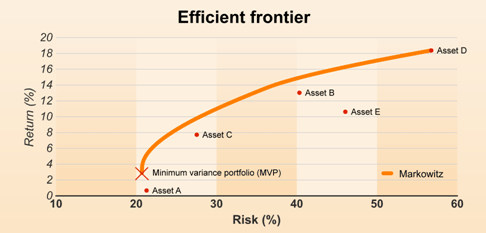
\includegraphics[width=0.9\textwidth]{efficient_frontier}
      \caption{Example of an Efficient Frontier Without a Risk-Free Asset \cite{efficient_frontier}.}
      \label{efficient_frontier}
    \end{figure}

    Each point on the line in Figure~\ref{efficient_frontier} represents a portfolio which is considered to be efficient (ie no other portfolio provides higher return without more risk and similarly for risk). In Figure~\ref{efficient_frontier} Assets A-E represent what the portfolio will be made out of. 

    Markowitz's model is subject to serous criticisms as stated in \cite{crit}, and the main ones being that a measure of dispersion can be adopted as a measure of risk only if the relevant distribution is symmetric. Another problem is that the distribution of individual asset returns has a tendency to show a higher probability of being fat-tailed. In case of non-normal, non-symmetric distributions, the utility function must be quadratic \cite{crit}. 

    This criteria should not be taken lightly since the assets' return does not follow normal distributions in real world situations \cite{non-dist}. This approach can only be used if the investor's utility function is quadratic with non-positive second derivatives or if the asset's return distribution can be fully described. Several research have indicated that that the quadratic utility function implies that beyond some level or return, marginal utility of the decision maker for wealth becomes negative \cite{crit2,crit3}. 
  % section markowitz_model (end)

  \section{Hill Climbing} % (fold)
  \label{sec:hill_climbing}
  Hill climbing \cite{hill,hill2} is an iterative optimisation algorithm which belongs to the family of local search. The algorithm must begin with an arbitrary solution to a problem, then attempts to find a better solution by incrementally changing single elements of the solution. It repeatedly iterates through new solution until no further improvements can be found. 

  The following pseudo-code is a basic hill climbing algorithm:

    \begin{algorithm}[H] \label{eq:hill}
      currentNode = startNode; \\
      \While{not endingCondition()}{
        L = NEIGHBORS(currentNode) \\
        nextEval = -INF \\
        nextNode = NULL \\
        \For{all x $\in$ L}{
          \If{EVAL(x) $>$ nextEval}{
            nextNode = x \\
            nextEval = EVAL(x) \\
          }
        }
        \If{nextEval $\leq$ EVAL(currentNode)}{return currentNode}
        currentNode = nextNode
      }
      \caption{Discrete Space Hill Climbing pseudo-code.}
    \end{algorithm}
  When local search algorithms, such as hill climbing, come across functions, such as $f(x)=\sum\limits_{i=1}^n -x_i sin(\sqrt{|x_i|})$ which was considered \cite{localmin} as a particularly hard function to optimise due to the number of local minima increases exponentially with the number of dimensions of the searching space, they very quickly and easily get trapped in a local optima. This is absolutely not acceptable, specially when there are hundreds of thousands of pounds at stake. 

  There are some improved hill climbing implementations \cite{hill3} where they force more randomness into the algorithm making it behave more like a genetic algorithm. The possibility of becoming stuck in a local optimal instead of the global is the biggest reason why I would choose PSO and other evolutionary algorithms over hill climbing. 

  Scalability is another major factor when considering an optimisation algorithm. Hill climbing will just not be able to cope with the amount of dimensions that the portfolio optimisation function belongs to. These are the biggest reasons why I have chosen not to use Hill climbing or similar local search algorithms. 

  % section hill_climbing (end)

  % \section{Alternative Optimisation} % (fold)
  % \label{sec:alternative_optimisation}
  %   Some other optimisation like simplex method or hopefully something better which is not as good at solving the portfolio optimisation problem as PSO is. 
  %   Hill climbing / greedy search - simplex - scalability problem on deterministic. Easy for hill climbing to get stuck in local opt
  % % section alternative_optimisation (end)

  %------------------------------------------------------------------
  % \section{Heuristic and Metaheuristic Algorithms} % (fold)
  % \label{sec:heuristic_and_metaheuristic_algorithms}
  %   The use of heuristics is very attractive to solve real world problems. For many problems, a heuristic algorithm may be the unique way to obtain good solutions in a reasonably short space of time. Meta-heuristics, a subfield of general heuristic strategies, includes stochastic components to utilize randomised search capabilities. 

  %   In real world applications, 

  % % section heuristic_and_metaheuristic_algorithms (end)
  %------------------------------------------------------------------

  % \section{Portfolio in Excel} % (fold)
  % \label{sec:portfolio_in_excel}
    
  % % section portfolio_in_excel (end)

  % \section{Something PSO} % (fold)
  % \label{sec:something_pso}
  
  % % section something_pso (end)

  % \section{PSO applied} % (fold)
  % \label{sec:pso_applied}
  
  % % section pso_applied (end)


\chapter{Problem Domain}

  In this chapter I will discuss some reasons why I believe this is a worth while project. I will mention what methods I intend to implement and for what reasons. It will then follow by a brief section describing my approach, although the full description of the actual approach taken is document in Chapter~\nameref{chap:design}.
  
  Particle Swarm Optimisation has already been effectively implemented to solved various optimisation problems \cite{pso_app,pso_app2,pso_app3} in variant domains such as biomedical, networks, clustering, finance, combinatorial optimisation and many more \cite{pso_app_main}. 

  This project mainly focuses on expanding the implementation created by Rabanal, Rodrıguez and Rubio in their paper ``A Functional Approach to Parallelize Particle Swarm Optimization'' and more importantly, its application to solve the portfolio optimisation problem \cite{marko2}. The optimisation algorithm has been successful by means of accuracy as well as efficiency \cite{haskellPSO}, and when millions of pounds are at stake, choosing the right portfolio to invest in is extremely important, meaning that choosing the right algorithm is even more crucial.

  \textbf{Why PSO.} I have chosen to use PSO as it is better than other familiar optimisation techniques such as the simplex method or hill climbing. It does not risk becoming stuck in local optima like the others. It out-performs the others with incredible efficiency when the optimisation function is over higher dimensional fields. 

  \textbf{Why Portfolio.} It is a fundamental problem in finance, making it an ideal candidate to test PSO's capabilities. As already mentioned, there is a lot of money at stake, so making tools which are efficient to help humans make these multi-million decisions would definitely be worth the hard work. After some brief searching, I noticed that there is not that much information in this field out there, making this a novel and exciting topic. This two-sided coherent risk measure is a well defined function and compatible with PSO function format. 

  \textbf{Why Haskell.} Firstly, Haskell is a passion for me, it has scared so many yet intrigues a few. Apart from its syntactical charm (subjective I know), there are many benefits, specially when working with mathematical applications. Haskell has been given by default to work with arbitrary large number calculation, this will help against overflow problems which are ever so common with most languages. The functional nature of Haskell makes it effortless to formulate complex mathematical equations \cite{haskellPSO}. Other extra influences are that it has a great online community, very friendly and helpful, or lazy evaluation and function and partial function composition. 

  % \begin{itemize}
  %   \item PSO
  %   \begin{itemize}
  %     \item Better than simplex at higher dimension optimisation
  %     \item Good at not becoming stuck in local optima
  %     \item Much better at optimisation than humans!!!
  %   \end{itemize}
  %   \item Portfolio
  %   \begin{itemize}
  %     \item Fundamental problem in finance
  %     \item Good to test PSO
  %     \item Loads of money at stake
  %     \item Not that much out there
  %     \item Suited well for PSO
  %   \end{itemize}
  %   \item Haskell
  %   \begin{itemize}
  %     \item Arbitrary large number calculation
  %     \item Functional nature is great for programming mathematical problems efficiently
  %     \item Lazy evaluation implies efficient use of resources
  %     \item Good online community
  %   \end{itemize}
  % \end{itemize}

  \section{Approach} % (fold)
  \label{sec:approach}
  This is a research project aimed at designing and evaluation a possible system to solve the portfolio optimisation problem through the use of particle swarm optimisation. A possible expansion to the PSO implementation \cite{haskellPSO} will also be considered and attempted. The new concept for improving the PSO implementation might be through the use of constriction factors and self-termination described in Chapter~\ref{chap:design}. Just as importantly as the optimisation method PSO, is was formulate the portfolio optimisation problem. I will follow closely a revolutionary way to measure a portfolio's risk \cite{two_sided_risk} written by Zhiping Chen. Although Chen completely rethinks the concept of measuring risk by taking into account both upside and downside risk, some work would have to be done to be able to turn this into a function which PSO will be able to handle as well as take into account the constraints which have to be satisfied. 

  As this is a research project for testing whether it is possible to solve the portfolio optimisation problem through PSO, the application will use simulation (offline) data instead of real-time streams. It is not too much a stretch of the imagination to be able to implement real-time processing as all the financial information is based on previous data. Changing a function, expected return for example, to recalculate its value after new data has come through would be trivial. 

  One of the main novelties of this project is the use of penalty functions in addition to the two-sided risk measure. The use of a penalty means one can formulate various constraints into a way that can be implemented for the PSO to understand. We use a penalty value to penalise any deviation from the constraint. This also means we need a way to turn deviation from the constraint into a distance measure, this is straight forward given the constraints are linear. 

  For further implementation and design details, including the reasoning behind the decision, please refer to \nameref{chap:design}.
  % section approach (end)


\chapter{Requirements}
This chapter describes the requirements for this project. Table~\ref{table:functionalRequirements} refers to the functional requirements from technical point of view. Section~\nameref{sec:non_functional} focuses on the non-functional requirements of the system.

  \section{Functional} % (fold)
  \label{sec:functional}
  \begin{table}[ht]
    \setlength{\extrarowheight}{2.0pt}
    \begin{tabular}{|l|l|l|}
      \hline
      No. & Description & Priority \\
      \hline
      \textbf{1} & \textbf{Optimisation of Portfolio} & \\
      \hline 
      \textbf{1.1} & \textbf{PSO} & \\
      \hline 
      1.1.1 & Initialisation of particle population & High \\
      \hline 
      1.1.2 & Processing swarm optimisation & High \\
      \hline 
      1.1.3 & Updating the local and global (at each step) particle values & High \\
      \hline 
      1.1.4 & Calculating an optimal solution & High \\
      \hline 
      1.1.5 & Presenting the results & Medium \\
      \hline 
      \textbf{1.2} & \textbf{Portfolio Optimisation} & \\
      \hline 
      1.2.1 & Minimise portfolio variance & High \\
      \hline 
      1.2.2 & Maximise portfolio expected return & Medium \\
      \hline 
      1.2.3 & Use multi-objective for optimum solution & Low \\
      \hline 
      1.2.4 & Refining results output & High \\
      \hline 
      1.2.5 & Make results for readable for user & High \\
      \hline 
      \textbf{2} & \textbf{User Input} & \\
      \hline
      2.1 & Allow the user to enter the name of the data file & High \\
      \hline
      2.2 & Allow the user to change the expected portfolio return & High \\
      \hline 
      2.3 & Allow the user to select the name for the output file & Medium \\
      \hline 
      2.4 & Allow the user to change the PSO particle size & Low \\
      \hline 
      2.5 & Allow the user to change the PSO iteration number & Medium \\
      \hline
      \textbf{3} &\textbf{Output format} & \\
      \hline 
      3.1 & Display the results during run-time & Medium \\
      \hline 
      3.2 & Make results more readable for output file & High \\
      \hline
      3.3 & Store results into a separate file & High \\
      \hline
    \end{tabular}
    \caption{Functional requirements for system.}
    \label{table:functionalRequirements}
  \end{table}
  % section functional (end)

  \section{Non-functional} % (fold)
  \label{sec:non_functional}
    As this system is an extension on a PSO module \cite{haskellPSO}, it is crucially important to devote a considerable amount of time to testing. This is to ensure that the alterations do not affect the performance of the overall efficiency of the algorithm and quality of the optimisation.  

    The system's scalability is something not to be overlooked. As each asset in a portfolio represents one dimension in the fitness function (not to be confused with just another linear factor of the same coefficient in a function), optimising a function in, for example, 100 dimensions (100 assets) might be to much for the system to cope with. 

    Running the PSO requires setting up various parameters and thresholds for optimisation (size of the particle population, number of iterations, inertia weights and convergence coefficients). These parameters need to be optimised for the algorithm to be computationally effective and produce accurate results. 
  % section non_functional (end)

\chapter{Risk Assessment}
Section~\ref{sec:social} and Section~\ref{sec:project_based} describe possible risks which might affect the development of the project and some worries which must not be overlooked.

  \section{Social Risk Assessment} % (fold)
  \label{sec:social}
    I do not refer to the term `Social' as a worry that I will be too sociable and not focus enough on my project. I simply mean ``stuff not directly to do with my project area''. The first thing that worries me is that I am reading a joint-honours degree in mathematics and computing science, almost all of my colleagues have nothing to do this term except their projects, where I have two more modules as well was this project. Most of them where smart enough to take an extra  ``padding'' module last term so they did not have to do anything else this term. I was unable to do that as I had to do my Mathematics dissertation and 3 other modules last term. 

    Doing a join-honours degree has meant I have gotten much more out of studying here than most people but it also means I have had to learn (in terms of quantity) much more material. I worry that having to do these other two mathematics modules this term might affect my project or \textit{visa-versa}. I plan to work as long as I can on all subjects even if it mean burning the candle at both ends as it were. Careful planning of my days will help and I hope it will be enough to achieve the grades I desire and require. 
  % section social (end)
  \section{Project Based Risk Assessment} % (fold)
  \label{sec:project_based}
    \subsection{Haskell} % (fold)
    \label{sub:haskell}
      The nature of Haskell, as mentioned in Section~\ref{sec:haskell} in Chapter~\ref{chap:background}, is strongly typed meaning that the type of a function (ie input an \textit{int} and return \textit{bool}) is very important. Because of this, expanding the PSO implementation by \cite{haskellPSO} will be much more work that on other less typed languages, do to cascading effect. Changing just one tiny part of a Haskell function will meaning altering any function which use this function. Fortunately, you can define partial functions and use these for partially giving function inputs as a sort of mathematical abstraction. This is very useful for defining function to be used as inputs for the PSO. 
    % subsection haskell (end)
    \subsection{PSO} % (fold)
    \label{sub:pso}
      One thing that is a worry whenever trying to optimise any function is the possibility of becoming stuck in a local optimum value, and then mistaking that as the global optimal best solution. Randomness is key when dealing with such situations. This problem is solved by introducing randomness, not only to each particle's momentum but also to the initialisation of the swarm itself. This ensures that the swarm is able to search the whole domain and then determine the optimal value.

      When evolutionary algorithms come across functions, such as $f(x)=\sum\limits_{i=1}^n -x_i sin(\sqrt{|x_i|})$ which was considered \cite{localmin} as a particularly hard function to optimise due to the number of local minima increases exponentially with the number of dimensions of the searching space, the danger might be that when it finds a certain local minima which might seem like a ``good enough'' solution, then the algorithm might converge to this false solution. Furthermore when what we are trying to optimise has local minima and global minima which differ by thousands of pounds worth of stocks when applied to financial situations it is crucial the algorithm does not get stuck in non-optimal solutions. 
    % subsection pso (end)
    \subsection{Portfolio} % (fold)
    \label{sub:portfolio}
      The current model has no notion of financial markets or knowledge of social economic climates, when the algorithm is given a portfolio to optimise, it will not look for or know of any problems that a company might be going through. It might be obvious that a company is going to crash any minute from now but if the system thinks, from previous financial data (and nothing more), that the company seems profitable then it will tell the user to invest in the company. One way to help this problem is introducing semantic web engineering into the system, this is not something I will be able to do or even look into in this project but the idea of it does seem both plausible and worth worth while for future developments.
    \subsection{Finance} % (fold)
    \label{sub:finance}
      This project required large amounts of finance background or knowledge. I have never studied or read any sort of financial theory or concepts. A worry is that I will have to learn more than the ideal amount when doing a short term project such as this, made even shorter by the amount of other modules I have to study at the same time, not to mention the time spent dealing with what to do in the future, ie. applying for jobs, masters etc.. 
    % subsection finance (end)
    % subsection portfolio (end)

  % section project_based (end)

\chapter{Methodology and Technologies}
  This chapter describes the methodology used in the project for the research, design, implementation and testing. It also mentions the technologies used to achieve the goals. 
  \section{Methodology} % (fold)
  \label{sec:methodology}
  This sections is basically an extension to the project plan which had to be made during the first week of the project. An approximate guideline to follow the project was set focusing on the project deadlines. I left a few weeks for margin for error in case something takes longer than planned, Figure~\ref{timline} shows the plan. 

  \begin{figure}[H]
      \centering
        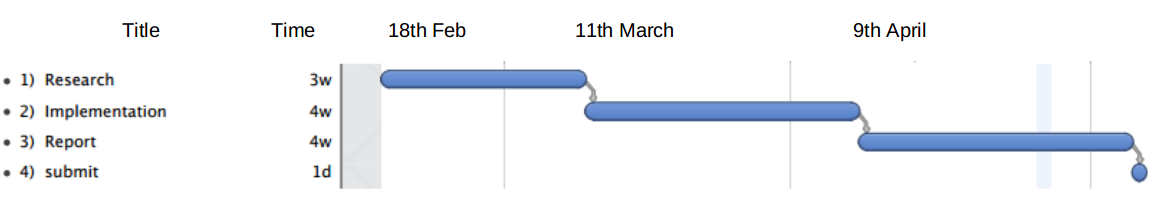
\includegraphics[width=0.9\textwidth]{time-line}
      \caption{Time line for project completion.}
      \label{timline}
  \end{figure}

  For this project to be successful I am planning on spending the initial weeks researching relevant literature and becoming familiar with the concepts of Particle Swarm Optimisation. This is a completely new field to me and understanding the key ideas and models will be critically important. Not only will I need to understand PSO's background I will also need to study previous implementations and applications in order to become absolutely comfortable with it. Finally, as I am planning on improving an existing algorithm, I will have to spend some time becoming familiar enough with the code so that I will be able to modify it with ease.

  The implementation stage will consist of designing the future system and the realisation of the plans. Key design decisions will have to be made during this stage and the solutions might be obtained from the analysis of previous work. 

  To complete this project I am going to test each function as I create or modified them, this will ensure a safe and stable system. This will be done to ensure that changes will not affect any previous functionality. The tests will evaluate the efficiency as well as the accuracy of my system. Given the nature of PSO's `random' initialisation of particles and their velocities,  I want to make sure that the results are consistent. 

  The writing of this result will be flexible, the sections will be written as needed or when the section arises naturally throughout the project. 

  % section methodology (end)

  \section{Technology} % (fold)
  \label{sec:technology}

    \subsection{Haskell} % (fold)
    \label{sub:haskell}
      Coming from a strong mathematical background I find functional languages easier to understand. Also one huge advantage of pure functional languages is that the absence of side-effects allow them to offer a clear semantic framework to analyse the correctness of programs. 

      As Haskell is the functional language I am more familiar with, I did not see the point in learning a new language as it would only restrict my project process, so Haskell was a clear winner. 

      There are other PSO implementations in other languages such as C and Ruby but as already mentioned, Haskell is my preferred language. 

    % subsection haskell (end)
    \subsection{Operating System} % (fold)
    \label{sub:operating_system}
    As Haskell is platform independent (in the sense that it can be compiled in Windows, Linux or Mac) I have chosen to use Ubuntu 12.04 as it is my preferred OS and I feel the most comfortable with it. In addition, I would not be affected in the about of software needed for the project as it is provided for all three OSs already mentioned. 

    The work was carried out on my personal laptop (Intel CORE$^{TM}$ i3 @ 2.6GHZ,4Gb RAM). If required due to any reasons, the university provide classroom PCs (Intel CORE$^{TM}$ i3-2100 CPU @3.10 GHz, 3 Gb RAM) although I have faith that my own machine will be reliable enough for me not to have to change machines. 
    
    Sublime Text 2 was chosen as the IDE for the project. It has many useful functions \cite{sublime} and similarly for the choice of OS, I am happy with this editor.
    % subsection operating_system (end)
  
  % section technology (end)

\chapter{System Design and Architecture}\label{chap:design}
This chapter describes the system's basic design and its program flow. As this project is partly an extension of an implementation of PSO \cite{haskellPSO}, Section~\ref{sec:original_pso_implementation} outlines the core architecture of that implementation in order to provide a base to the changes made in this project. Section~\ref{sec:expansion_for_portfolio_optimisation} explains the design and ideas behind the system's modification and further design on how to apply the algorithm to solve the portfolio optimisation problem.

  \section{Original PSO Implementation} % (fold)
  \label{sec:original_pso_implementation}

    \subsection{Initialisation} % (fold)
    \label{sub:initialisation}
    The main purpose of this stage is to create a population of particles (called a swarm) which will be used to search the domain and find the optimal solution to our problem. The application uses a function called \textit{initialise} to randomly create a list of initial particles to populate the search space. It is written in accordance with Algorithm~\ref{eq:pso} and thanks to Haskell's well designed and efficient random generators \cite{random} it ensures that the particles are initialised in such a way to exploit the search space well. For details, see Algorithm~\ref{eq:pso}. After the population has been initialised, the algorithm moves on to the optimisation phase.
    % subsection initialisation (end)
    \subsection{Inertia Weights} % (fold)
    \label{sub:inertia_weights}
    PSO relies on randomness, as in Equation~(\ref{eq:vel}). As this project is not intended to experiment much with the basic PSO parameters we will use the inertia weights presented in \cite{constriction_factor_3}. If there is enough time, we may wish to experiment with different weights. This does not mean that testing will not be done, it just means that we will not deviate from our goal to look into this matter, as so much research has already been done\cite{inertia}.
    % subsection inertia_weights (end)
    \subsection{Optimisation} % (fold)
    \label{sub:optimisation}
    The core function dealing with the optimisation is done by ``steps'' or iterations, at each iteration a particle is updated by a function \textit{updateParticle} in accordance to Equation~(\ref{eq:vel}) which changes the position and velocity. The same function checks whether the new position is better that the best solution so far. A boolean system is used, if the new position of the particles is better that global best position, then this position will become the new global best position. This is done recursively until all the particles in the swarm have been updated. A function had to be created to deal with the comparison of particles' results and both the position and the value of that position are stored for each particle. 

    For any more details on how the optimisation is done, please refer to \nameref{sec:particle_swarm_optimisation} in Chapter 2.
    % subsection optimisation (end)
    \subsection{Termination} % (fold)
    \label{sub:termination}
    A function was created to deal with the termination, a user specifies the number of iterations (``steps'') that the algorithm is allowed to run for. This independent function is simple, it runs recursively, applying one \textit{updateParticle} at a time and terminates once there are no more iterations to be performed and returns both the value of the global best and its position. 
    % subsection termination (end)
  % section original_pso_implementation (end)

  \section{Expansion for Portfolio Optimisation} % (fold)
  \label{sec:expansion_for_portfolio_optimisation}

    \subsection{Interface and User Input} % (fold)
    \label{sub:interface_and_user_input}
    The original implementation needed the swarm size and number of iterations to be hard-coded into the algorithm. This model allows the user to specify how many particles they would like as well as how many iterations the PSO should run for. I do not think the user should be allowed to set the inertia weights as they might not fully understand their purpose and therefore give non-optimal inputs.
    % subsection interface_and_user_input (end)
    \subsection{Data (asset) file} % (fold)
    \label{sub:data_file}
    The user will have to input a file with the assets' information in order for the system to optimise a portfolio. There is no standard format for such a file and it really is up to preference. I have decided to arrange the file as follows: ``Name Rate-Of-Return Expected-Required-Return'', where \textit{Name} is the company's name (either full or the ticker label ie Google vs GOOG), \textit{Rate-Of-Return} is the company's rate of return and \textit{Expected-Required-Return} is the expected required return of the same company. I will set it so that each company is has its own line to make it easier for the user to view and edit the asset file.

    Figure~\ref{fig:asset_file} shows an example file containing a selection of assets which the user wants to maximise for their portfolio. As you can see the first item is the name of the company, followed by a single space and then the rate of return, another space and the expected return. Each company has their own line and they can have as many companies as they would like. 
    \begin{figure}[H]
      \centering
        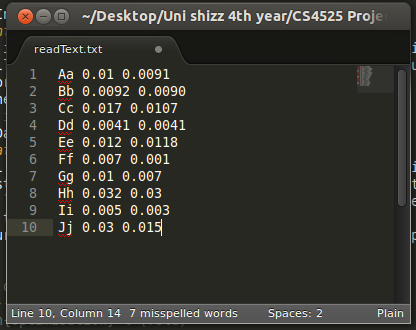
\includegraphics[width=0.7\textwidth]{asset-file}
      \caption{Example File of Assets.}
      \label{fig:asset_file}
    \end{figure}
    % subsection data_file (end)
    % ----------------------------------------------------
    % \subsection{Optimisation} % (fold)
    % \label{sub:optimisation}
    
    % % subsection optimisation (end)
    % ----------------------------------------------------
    \subsection{Constriction Factor} % (fold)
    \label{sub:constriction_factor}
    Maurice Clerc in his study on stability and convergence of PSO \cite{constriction_factor} has introduced the concept of a constriction factor. Clerc indicated that the use of a constriction factor may be necessary to insure convergence of the PSO for certain fitness functions.

    In order to ensure convergence of the PSO, the velocity from Equation~(\ref{eq:vel}) can be expressed as follows:
    \begin{equation} \label{eq:cf}
      \begin{split}
        V_{i}^{t+1} & = K \Bigg[ V_{i}^{t} + c_1 r_1 \times \Big( Pbest_{i}^{t} - X_{i}^{t} \Big) + c_2 r_2 \times \Big( Gbest^{t} - X_{i}^{t} \Big) \Bigg] \\
        \text{where }\\
        K & = \frac{2}{\mid 2 - \phi - \sqrt{\phi^2 -4\phi} \mid} \text{ and } \phi = c_1 + c_2 \text{ s.t. } \phi > 4  \\
        % \text{and} \\
        % \phi = c_1 + c_2 , \phi > 4 \\
      \end{split}
    \end{equation}

    The convergence characteristic of the system can be controlled by $\phi$ through choosing suitable $c_1$ and $c_2$ in \eqref{eq:cf}. In this approach, $\phi$ must be greater than 4 to guarantee stability \cite{constriction_factor_2}.
    % subsection constriction_factor (end)
    \subsection{Termination} % (fold)
    \label{sub:termination}
    If time allows, it would be nice to have a self-termination PSO which, no matter how many iterations are left, terminates if it thinks that the optimal solution is reached. This could be done by the concept of a threshold, if all the solution reach this threshold, then there is no point in carrying on. For example, if all the solution are close enough to each other for a long period of iteration, say $10^{-10}$ within 100 iterations, then there is no point in looking for thousands more iterations just to find something which will not affect the outcome. 

    In order to achieve this, we would need three extra parameters to be added, one to define the threshold, another one to define the maximal number of iterations allowed without improvement (call this \textit{mni}, and another one to compute the current number of remaining iterations allowed without improvement(call this \textit{cni}. After each call to the updating function, compare the current best solution to the past best solution to decide whether there has been a relevant improvement or not. The algorithm would either change the number of iterations to \textit{mni} (in case there was relevant improvement), otherwise reduce the value of \textit{cni} by one. 
    % subsection termination (end)
    \subsection{Fitness Function} % (fold)
    \label{sub:fitness_function}
    Due to the nature of Haskell and with some mathematical background it is very straight forward and logical to create a function to represent the measure of risk, namely $\rho_{a,p}(R)$ in Equation~(\ref{eq:portfolio-risk}) in Section~\nameref{sec:portfolio_management} Chapter~\ref{chap:background}. What is much more challenging, is finding a way to include the constraints in Equation~(\ref{eq:portfolio-risk-constraints}) in a way that the algorithm can deal with the main function without violating these condition. Two methods were considered, using multi-objective optimisation or a penalty function. Due to the constraints being linearly-independent, it will be straight forward to affect the optimal solution through factors of the constraints. The design of this will be described next, in the following Subsection~\ref{sub:penalty_function}.
    % subsection fitness_function (end)
    \subsection{Penalty function} % (fold)
    \label{sub:penalty_function}
    One of the most straight forward approaches, in my opinion and possibly due to strong background in measure theory, to solving constrained optimization problems is the use of a penalty function\cite{constraint}. Using such an approach means transforming the optimisation problem, such our $\rho_{a,p}(R)$ in Equation~(\ref{eq:portfolio-risk}), to include the behaviour of being ``punished'' if the constraints are not met. One can construct a single new objective function from combining $\rho_{a,p}(R)$ plus linear factors of the differences of each constraint in Equation~(\ref{eq:portfolio-risk-constraints}), this new objective function will be used to find an optimum value for the portfolio problem. Thus a new optimisation function can be created:
      \begin{equation} \label{eq:unconstraint-portfolio-risk}
        \begin{split}
          \text{min } f(R) & \\
          \text{where } 
          f(R) & = \rho_{a,p}(R) + \frac{1}{\delta}|\widehat{R}-\eta| + \frac{1}{\delta}|\sum\limits_{i=1}^N x_i -1| \\
          % \rho_{a,p}(R) & = a \|(R-\widehat{R})^+\|_1 + (1-a)\|(R-\widehat{R})^-\|_p - \widehat{R} \\
        \end{split}
      \end{equation}
    Now an explanation on what is happening in Equation~(\ref{eq:unconstraint-portfolio-risk}). Firstly,$\delta > 0$ is called the penalty parameter and $\frac{1}{\delta}$ is called the penalty value \cite{constraint}. The penalty parameter should be small enough so that whenever a constraint is violated, the penalty value will be big enough to affect the result of the solution. Secondly, the use of absolute values refers to the distance traveled from the desired value, for example if the sum of the weights is not equal to 1 then $|\sum\limits_{i=1}^N x_i -1| > 0$ multiplying this by a strong enough penalty value will ensure that the solution will not be taken as an optimal one. Finally, a similar method is used for deviating from the required expected return. 

    One may notice that in this new optimisation function, the lower and upper bounds for how much one can invest in each asset are not included. This is due to how PSO handles search space domains and will be explained in the following Subsection~\ref{sub:forced_diversification}.
      % \begin{equation} \label{eq:portfolio-risk}
      %   \begin{split}
      %     \rho_{a,p}(R) & = a \|(R-\widehat{R})^+\|_1 + (1-a)\|(R-\widehat{R})^-\|_p - \widehat{R} \\
      %   \end{split}
      % \end{equation} 
      % Now that there is a way to measure risk, the portfolio optimisation problem can be formulated as follows:
      % \begin{equation} \label{eq:portfolio-risk-min}
      %   \begin{split}
      %     \text{min } \rho_{a,p}(R) \\
      %   \end{split}
      % \end{equation} 
      % Subject to constraints:
      % \begin{equation} \label{eq:portfolio-risk-constraints}
      %   \begin{split}
      %     \widehat{R} = \eta \\
      %     \sum\limits_{i=1}^N x_i = 1 \\
      %     l_i \leq x_i \leq u_i
      %   \end{split}
      % \end{equation}
    % subsection penalty_function (end)
    \subsection{Forced Diversification} % (fold)
    \label{sub:forced_diversification}
    Equation~(\ref{eq:unconstraint-portfolio-risk}) did not include lower and upper limits for each assets as in Equation~(\ref{eq:portfolio-risk-constraints}), this is because the implementations \cite{haskellPSO} already takes into account bounds for the solution's domain for a given fitness function. Since our objective is to find weights for each asset, the number of assets is the domain for our fitness function. So the bounds for the proportions can be set within the algorithm's parameters.

    The bounds inside the algorithm can be used to give a sense of diversification \cite{diversification}, by not allowing how much you invest on each asset to be too small or to large. For example, you might specify that you have to invest at least 5\% and at most 50\% of any asset in a portfolio, this forces the investor to consider at all assets and helps lowering the risk of a portfolio \cite{diversification}.
    
    % subsection forced_diversification (end)
    \subsection{Presenting the Results} % (fold)
    \label{sub:presenting_the_results}
    After the algorithm has finished, the results are displayed on the screen and saved in a separate file which will be called ``output-DATE'', where date is in (year,month,day) format, for example ``output-2014,3,15''. If there is multiple runs in one day, the new results are added to the end of that same file.
    % subsection presenting_the_results (end)
  % section expansion_for_portfolio_optimisation (end)


% \chapter{Financial Data}
%   \section{Data Description} % (fold)
%   \label{sec:data_description}
  
%   % section data_description (end)

%   \section{Problem Domain} % (fold)
%   \label{sec:problem_domain}
  
%   % section problem_domain (end)

%   \section{Assets and their Weights} % (fold)
%   \label{sec:assets_and_their_weights}
  
%   % section assets_and_their_weights (end)

%   \section{Analysis} % (fold)
%   \label{sec:analysis}
  
%   % section analysis (end)

%   \section{PSO Parameters} % (fold)
%   \label{sec:pso_parameters}
  
%   % section pso_parameters (end)

%   \section{Experimentation and Testing} % (fold)
%   \label{sec:experimentation_and_testing}
  
%   % section experimentation_and_testing (end)

%   \section{Portfolio Constraints} % (fold)
%   \label{sec:portfolio_constraints}
  
%   % section portfolio_constraints (end)

%   \section{Results} % (fold)
%   \label{sec:results}
  
%   % section results (end)

\chapter{Experimentation and Testing}
This chapter shows the results of some of the tests I made, during the implementation I tested every function independently and then tested the full program after all the sub-programs where merged together. This project is not primarily about testing the PSO algorithm, it's more about testing whether we can use it to solve the portfolio selection problem and whether it's safe to use. 

I condensed greatly the amount of data collected. I ran many tests, within each test there were many sub-test and each sub-test was ran 30 times. From this I calculated means and standard deviations which are used to give readable results. Overall there are about 7 files which represent test cases, each file contains the results for the sub-tests all grouped together and these files are each about 500 lines long.  
  \section{Scalability} % (fold)
  \label{sec:scalability}
    Unfortunately, I hindered the system by insisting that the minimum percentage of any asset in the portfolio is 5\% and the maximum is 35\%. This means that after 20 assets, the system stops giving credible results, as you can notice, if we have 21 assets and each one has to be at least 5\%, then we will end up have 105\%, which of course makes no sense. It will be essential to implement a better diversification technique if I plan to consider a large amount of assets. 

    This problem has nothing to do with the PSO algorithm, the algorithm has proven to be efficient even around 60 dimensional search spaces, this depends on the nature of the optimisation function of course. 
  % section scalability (end)

  \section{Precision} % (fold)
  \label{sec:precision}
  These tests should verify that the system is stable, by this I mean that given the same input, the output should be almost the same. A there is a lot of randomness in the algorithm, one can not expect the outputs to be equal, but they should be equivalent up to some threshold. In this case the threshold will be $1.0\times10^{-8}$, this small enough to not affect the expected return from a optimised portfolio. 

    \subsection{Testing Strategy} % (fold)
    \label{sub:testing_strategy}
      I will run nine tests and record the expected rate of return for the solution the algorithm gives. Each of the nine tests will be run 30 times with a mean and standard deviation calculated and shown in the following sections. The nine tests will be as follows:
        \begin{itemize}
          \item Test 1: PSO 20 particles, 100 iterations, 5 assets
          \item Test 2: PSO 20 particles, 300 iterations, 5 assets
          \item Test 3: PSO 40 particles, 100 iterations, 5 assets
          \item Test 4: PSO 20 particles, 100 iterations, 7 assets
          \item Test 5: PSO 20 particles, 300 iterations, 7 assets
          \item Test 6: PSO 40 particles, 100 iterations, 7 assets
          \item Test 7: PSO 20 particles, 100 iterations, 10 assets
          \item Test 8: PSO 20 particles, 300 iterations, 10 assets
          \item Test 9: PSO 40 particles, 100 iterations, 10 assets
        \end{itemize}
    % subsection testing_strategy (end)

    \subsection{Hypothesis} % (fold)
    \label{sub:hypothesis}
      My hypothesis is that the application is reliable and that the results (for the same input) will have almost the same output, ie it is reliable and precise, up to the threshold already stated. 
    % subsection hypothesis (end)

    \subsection{Results} % (fold)
    \label{sub:results}
      Table~\ref{table:expected_results} show the results for the 9 tests.
        \begin{table}[H]
          \setlength{\extrarowheight}{2.0pt}
          \begin{tabular}{|l|l|l|}
            \hline
            Test & Mean Result & Standard deviation \\
            \hline
            Test 1 & 0.0447 & $6.13954\times10^{-11}$ \\
            \hline
            Test 2 & 0.0447 & $1.58041\times10^{-17}$ \\
            \hline
            Test 3 & 0.0447 & $7.18283\times10^{-13}$ \\
            \hline
            Test 4 & 0.0527 & $3.3924\times10^{-10}$ \\
            \hline
            Test 5 & 0.0527 & $1.41115\times10^{-16}$ \\
            \hline
            Test 6 & 0.0527 & $6.83323\times10^{-13}$ \\
            \hline
            Test 7 & 0.101475 & $0.00279292$ \\
            \hline
            Test 8 & 0.1007 & $2.30303\times10^{-12}$ \\
            \hline
            Test 9 & 0.1007 & $2.56085\times10^{-11}$ \\
            \hline
          \end{tabular}
          \caption{Results for \nameref{sec:precision}, expected return.}
          \label{table:expected_results}
        \end{table}
      As you can see from Table~\ref{table:expected_results} all of the standard deviations are less than $1.0\times10^{-8}$ which was our threshold, except Test 7. This is a very good sign as we have only given PSO 100 iterations to complete its task and when we increase this to 300, the results are by far below the threshold. 

      The only reason Test 7 did not pass is because increasing the number of assets to 10 whilst only letting the algorithm run for 100 steps and only 20 particles was just to much. Remember that each asset represents a dimension, so in Test 7, the algorithm have 100 steps with 20 agents to search for an optimal value in a 10 dimensional search space.
    % subsection results (end)

    \subsection{Conclusion} % (fold)
    \label{sub:conclusion}
    From the results and our test strategy, we can conclude that the algorithm is reliable by means of precision. To be safe, we will have a minimum cap of 100 particles and 1000 iterations. This will be enough to ensure consistency for the average investment manager.       
    % subsection conclusion (end)
  % section precision (end)

  \section{Constriction Factors} % (fold)
  \label{sec:constriction_factors}
  In System Design and Architecture~\ref{sub:constriction_factor} the concept of a constriction factor was introduced. 
    
    \subsection{Testing Strategy} % (fold)
    \label{sub:testing_strategy}
      I plan to test whether this will in fact affect the outcome of the algorithm when applied to the portfolio optimisation problem, furthermore if it does affect it, then whether it improves or worsens the result. In order to test this I will conduct six different experiments, three without a constriction factor where one has the adjustment parameters taken from \cite{constriction_factor_3}, one with the two randomness coefficients that add up to less than 4 and one where they add up to more than 4, the importance of 4 can be read in \cite{constriction_factor}. Then three more with a constriction factor and the rest is the same as the previous three.

      All tests will run 20 times and the results and the time taken will be recorded, all tests will be set to 50 particles, 500 iterations and 10 assets. A mean result and standard deviation will be computed to be able to compare the results. This will give enough indication on how the constriction factor affects the fitness function and how it differs under various criteria.  
    % subsection testing_strategy (end)

    \subsection{Hypothesis} % (fold)
    \label{sub:hypothesis}
      Constriction factor when applied to the portfolio selection problem with appropriate coefficients will not improve the portfolio selection problem.
    % subsection hypothesis (end)

    \subsection{Results} % (fold)
    \label{sub:results}
      This subsection shows the results and the following Table~\ref{table:constriction_factor_results} contains the exact values for the results in my experiment, it will follow a short explanations of the results. 

      Firstly, the time it took for each test to run and there was no significant difference between them. Having a constriction factor did not affect the time it takes for the algorithm to complete. 

        \begin{table}[H]
          \setlength{\extrarowheight}{2.0pt}
          \begin{tabular}{|l|l|l|}
            \hline
            Test & Mean Result & Standard deviation \\
            \hline
            WO-CF Pefersen & 0.914099 & $1.61088\times10^{--16}$ \\
            \hline
            WO-CF $<$ 4 & 0.914099 & $1.72748\times10^{-16}$ \\
            \hline
            WO-CF $>$ 4 & 0.9141 & $5.36229\times10^{-6}$ \\
            \hline
            W-CF Pefersen & 0.91415 & 0.0000389374 \\
            \hline
            W-CF $<$ 4 & 0.91416 & 0.0000448388 \\
            \hline
            W-CF $>$ 4 & 0.914099 & $2.81328\times10^{-16}$ \\
            \hline
          \end{tabular}
          \caption{Results for \nameref{sec:constriction_factors}.}
          \label{table:constriction_factor_results}
        \end{table}

      Table~\ref{table:key_constriction_factor_results} shows what the acronyms in Table~\ref{table:constriction_factor_results} mean. 

        \begin{table}[H]
          \setlength{\extrarowheight}{2.0pt}
          \begin{tabular}{ l l }
            WO-CF Pefersen & : Without constriction factor and Pefersen coefficients  \\
            WO-CF $<$ 4 & : Without constriction factor and $\phi < 4$ \\
            WO-CF $>$ 4 & : Without constriction factor and $\phi > 4$ \\
            W-CF Pefersen & : With constriction factor and Pefersen coefficients  \\
            W-CF $<$ 4 & : With constriction factor and $\phi < 4$ \\
            W-CF $>$ 4 & : With constriction factor and $\phi > 4$ \\
          \end{tabular}
          \caption{Key for \nameref{table:constriction_factor_results}.}
          \label{table:key_constriction_factor_results}
        \end{table}

      The reason for using Pefersen coefficients is stated in the design and architecture section of this report, \nameref{eq:cf} in \nameref{sec:original_pso_implementation}. One can see from Table~\ref{table:constriction_factor_results} that importance having $\phi > 4$ when introducing the constriction factor, in W-CF Pefersen and W-CF $<$ 4 one can see a serious decrease in the optimum found. 

      What is interesting here is that PSO for the fitness function is efficient and consistent without the constriction factor as shown in Table~\ref{table:constriction_factor_results} where WO-CF Pefersen and WO-CF $<$ 4 both have the same mean and almost exact standard deviation, meaning they behave the same. Once we introduce the constriction factor, it is almost catastrophic if we do not have $\phi > 4$, as both W-CF Pefersen and W-CF $<$ 4 have less efficient means and huge standard deviations (in comparison to the other tests) meaning they are unstable and unreliable. Once we make $\phi > 4$, the algorithm settles back to normal but does display higher standard deviation. 
    % subsection results (end)
    \subsection{Conclusion} % (fold)
    \label{sub:conclusion}
      Constriction factor when applied to the portfolio optimisation problem does not improve the results as in the hypothesis. It makes the results more unstable, the algorithm will therefore not include a constriction factor. 

      The use of the constriction coefficient can be viewed as a recommendation to the particle to ``take smaller steps''\cite{constriction_factor_4}, because of this it exploits optimal solutions, which is fine if there are not many, but it does mean that it travels less in the same amount of time. This is one of the main reasons why it did not improve the results. One has to bare in mind that each asset adds a dimension to out search space, this increases domain exponentially so as you increase the amount of assets in a portfolio coupled with making the PSO take smaller steps results in a much larger search space and less area covered by the end of the algorithm. 
       
    % subsection conclusion (end)

      % \begin{align}
      %   V_{i}^{k+1} & = K \Bigg[ V_{i}^{k} + c_1 r_1 \times \Big( Pbest_{i}^{k} - X_{i}^{k} \Big) + c_2 r_2 \times \Big(Gbest_{i}^{k} - X_{i}^{k} \Big) \Bigg] \\
      %   \text{where } \\
      %   K & = \frac{2}{\mid 2 - \phi - \sqrt{\phi^2 -4\phi} \mid}  \\
      % \end{align}

  % section constriction_factors (end)

  \section{Penalty value} % (fold)
  \label{sec:penalty_value}
  This experiment will see what happens with different penalty parameters. The penalty value, as explained in Section~\ref{sub:penalty_function} from Chapter~\ref{chap:design} is what ensures that the constraints in Equation~(\ref{eq:portfolio-risk-constraints}) are not violated. If the penalty is too small, it will not ensure that the constraints are kept, but if it is to large, then it might not let the algorithm settle on the optimal solution. The aim is to find a suitable penalty parameter. 

    \subsection{Testing Strategy}
      There will be 3 tests, each test will be run 30 times and an average and standard deviation calculated. This should ensure enough range to be able to find an adequate value.
      \begin{itemize}
        \item Test 1: PSO 100 particles, 1000 iterations, 10 assets, Pen Val = 0.01
        \item Test 2: PSO 100 particles, 1000 iterations, 10 assets, Pen Val = 0.1
        \item Test 3: PSO 100 particles, 1000 iterations, 10 assets, Pen Val = 1.0
      \end{itemize}

    \subsection{Hypothesis}
    Induced suspect that if the penalty value is to high, then the fitness function will be penalised to severely resulting in more `erratic' behaviour, it will be hard for the algorithm to settle down and find the global optimum. On the other hand, if it is too low, it will not penalise the function enough when it deviates from the constraints and may return optimal values which are incorrect. 

    \subsection{Results}
    As you can see from Table~\ref{table:penalty_results}, having the penalty parameter equal 1.0 in Test 3, is too big, resulting in a non-optimal solution by quite a bit although, from the standard deviation we can see that it is more stable (consistence/precise) than the other tests.
      % Table~\ref{table:penalty_results} shows the results. 
        \begin{table}[H]
          \setlength{\extrarowheight}{2.0pt}
          \begin{tabular}{|l|l|l|}
            \hline
            Test & Mean Result & Standard deviation \\
            \hline
            Test 1 & 0.100699 & $3.5\times10^{-13}$ \\
            \hline
            Test 2 & 0.100699 & $3.5\times10^{-11}$ \\
            \hline
            Test 3 & 0.100669 & $2.7\times10^{-15}$ \\
            \hline
          \end{tabular}
          \caption{Results for \nameref{sec:penalty_value}.}
          \label{table:penalty_results}
        \end{table}

      The question now is whether it is better to have a penalty parameter of 0.1 or 0.001. Test 1 vs Test 2: they have the same mean but Test 1 has a smaller standard deviation. This means that both Test 1 and Test 2 provide in average the same result, but Test 1 is more consistent.

    \subsection{Conclusion}
      For the reasons presented in the results, having the penalty parameter at 1.0 is too big, having it at 0.01 is too small and thus the penalty parameter will be held at 0.1. This should ensure consistent and reliable optimal solution to our portfolio optimisation problem.
  % section penalty_value (end)  

  \section{Parameter Investigation} % (fold)
  \label{sec:relationships}
  This test might seem a little peculiar at first but be assured, there is method in my madness. I want to see what the relationship is (if any) between the time it takes to run, the number of particles, number of iterations and number of assets.

    \subsection{Testing Strategy} % (fold)
    \label{sub:testing_strategy}
      I will run nine tests and record the time it takes to finish and the results just to make sure they are consistent. Each of the nine tests will be run 20 times with a mean and standard deviation calculated and shown in the following sections. The nine tests will be as follows:
        \begin{itemize}
          \item Test 1: PSO 20 particles, 250 iterations, 5 assets
          \item Test 2: PSO 20 particles, 500 iterations, 5 assets
          \item Test 3: PSO 40 particles, 250 iterations, 5 assets
          \item Test 4: PSO 20 particles, 250 iterations, 7 assets
          \item Test 5: PSO 20 particles, 500 iterations, 7 assets
          \item Test 6: PSO 40 particles, 250 iterations, 7 assets
          \item Test 7: PSO 20 particles, 250 iterations, 10 assets
          \item Test 8: PSO 20 particles, 500 iterations, 10 assets
          \item Test 9: PSO 40 particles, 250 iterations, 10 assets
        \end{itemize}
    % subsection testing_strategy (end)

    \subsection{Hypothesis} % (fold)
    \label{sub:hypothesis}
    There is no hypothesis here, I hope that there is no exponential relationship between increase in assets to increase in time for PSO to finish. The point of this exercise is to see if anything interesting happens. 
    % subsection hypothesis (end)

    \subsection{Results} % (fold)
    \label{sub:results}
      Table~\ref{table:sum_weight_results} show that even after 250 iterations, the algorithm already meets the constraints which where applied though a penalty function. This is indeed a promising result.
        \begin{table}[H]
          \setlength{\extrarowheight}{2.0pt}
          \begin{tabular}{|l|l|l|}
            \hline
            Test & Mean Result & Standard deviation \\
            \hline
            Test 1 & 1 & 0 \\
            \hline
            Test 2 & 1 & 0 \\
            \hline
            Test 3 & 1 & 0 \\
            \hline
            Test 4 & 1 & 0 \\
            \hline
            Test 5 & 1 & 0 \\
            \hline
            Test 6 & 1 & 0 \\
            \hline
            Test 7 & 1 & 0 \\
            \hline
            Test 8 & 1 & 0 \\
            \hline
            Test 9 & 1 & 0 \\
            \hline
          \end{tabular}
          \caption{Results for \nameref{sec:relationships}, sum of weight.}
          \label{table:sum_weight_results}
        \end{table}
      Table~\ref{table:time_results} show even the most computationally demanding process of optimising in $10^{th}$ dimensional space takes less than a fifth of a second. This is using a standard dual-core machine. I imagine using a specialised server will make the algorithm much faster. 
        \begin{table}[H]
          \setlength{\extrarowheight}{2.0pt}
          \begin{tabular}{|l|l|l|}
            \hline
            Test & Mean Result & Standard deviation \\
            \hline
            Test 1 & 0.0463947 & 0.00487954 \\
            \hline
            Test 2 & 0.107632 & 0.00912289 \\
            \hline
            Test 3 & 0.0812466 & 0.00542592 \\
            \hline
            Test 4 & 0.0555938 & 0.00491575 \\
            \hline
            Test 5 & 0.1253 & 0.00699414 \\
            \hline
            Test 6 & 0.106167 & 0.00669427 \\
            \hline
            Test 7 & 0.089034 & 0.00856579 \\
            \hline
            Test 8 & 0.181696 & 0.00828043 \\
            \hline
            Test 9 & 0.17403 & 0.00557404 \\
            \hline
          \end{tabular}
          \caption{Results for \nameref{sec:relationships}, time to finish.}
          \label{table:time_results}
        \end{table}
      Table~\ref{table:expect_return_results} show the expected return results for the optimal portfolio selected by the PSO algorithm.
        \begin{table}[H]
          \setlength{\extrarowheight}{2.0pt}
          \begin{tabular}{|l|l|l|}
            \hline
            Test & Mean Result & Standard deviation \\
            \hline
            Test 1 & 0.0447 & $6.13954\times10^{-11}$ \\
            \hline
            Test 2 & 0.0447 & $1.58041\times10^{-17}$ \\
            \hline
            Test 3 & 0.0447 & $7.18283\times10^{-13}$ \\
            \hline
            Test 4 & 0.0527 & $3.3924\times10^{-10}$ \\
            \hline
            Test 5 & 0.0527 & $1.41115\times10^{-16}$ \\
            \hline
            Test 6 & 0.0527 & $6.83323\times10^{-13}$ \\
            \hline
            Test 7 & 0.101475 & $0.00279292$ \\
            \hline
            Test 8 & 0.1007 & $2.3030\times10^{-12}$ \\
            \hline
            Test 9 & 0.1007 & $2.56085\times10^{-11}$ \\
            \hline
          \end{tabular}
          \caption{Results for \nameref{sec:relationships}, expected return.}
          \label{table:expect_return_results}
        \end{table}
    % subsection results (end)

    \subsection{Conclusion} % (fold)
    \label{sub:conclusion}
      As already mentioned, this section is intended to find anything (if any) interesting. The first thing I notice is the disproportional change in the results when increasing the number of iterations to the number of particles. By this I mean that Test 1 in Table~\ref{table:expect_return_results} has the same mean at Test 2 and Test 3, but the difference in output is not proportional to the change in input. From Test 1 to Test 2 and increase of doubling the number of iterations results in an decrease of about 50\%, whereas the difference between Text 1 and Test 3 is doubling the number of particles in a swarm which results in a decrease of around 20\%. 

      This leads me to think that if one had to between a large swarm or a large number of iterations for the algorithm, a larger number of iterations will be more beneficial. 

      Something which might not be completely straight forward is how increasing the number of particles increasing the time it takes for the algorithm to finish, even though it is based on the number of iterations. The reason for this is that at each iteration, the algorithm has to update every particles, meaning that if there are more particles, each iteration takes longer to complete, thus the whole algorithm takes longer to finish.
    % subsection conclusion (end)
  % section relationships (end)

  % \section{Risk and Risk Aversion} % (fold)
  % \label{sec:risk_and_risk_aversion}

  %   \subsection{Testing Strategy}
  %     The application will be run

  %   \subsection{Hypothesis}

  %   \subsection{Results}

  %   \subsection{Conclusion}

  %   Level of riskiness
  % % section risk_and_risk_aversion (end)


\chapter{Future Work}

  \section{PSO} % (fold)
  \label{sec:pso}
  This section mentions some future improvements or suggestions to improve the particle swarm optimisation algorithm.
    \subsection{Inertia weights} % (fold)
    \label{sub:inertia_weights2}
      Something to look into for the future, is whether changing the inertia weights will improve PSO on solving the portfolio optimisation problem. Some testing will need to be made to find the optimal inertia weights. Other things to consider is dynamic inertia weights as introduced in \cite{dynamic_inertia} or possibly decreasing inertia weight as in \cite{inertia}. It states that a weight of 1.9 encourages a better global search but a weight of 1.5 would be better for exploiting optima, having a continuously decreasing inertia weight from 1.9 to 1.5 might provide good guidelines for PSO to find all optima and then exploit the global optimum once the inertia weight settles. 
    % subsection inertia_weights (end)
    \subsection{Parallel Programming} % (fold)
    \label{sub:parallel_programming}
      One of the benefits of Haskell -- Functional stuff...
      Yet another benefit of Haskell is that through function abstraction \cite{haskellPSO} one can split the PSO algorithm into different processes. What takes the longest in PSO is updating each particles after every iteration, through parallel processes one can split the updating process into different sub-processes and computing them in parallel, improving the speed even more. Eden \cite{eden,eden2} is a parallel extension for Haskell, this would be what I would choose to implement parallel processing into the system.
    % subsection parallel_programming (end)
    \subsection{Self-termination} % (fold)
    \label{sub:self_termination}
      This might be beneficial for making the algorithm more efficient. Why should the algorithm run for $x$ amount of iterations if it will not improve the solution. There is no reason what so ever, the counter-positive though, might be crucial when calculating a portfolio's risk. There is the possibility that the share price has changes by the end of the algorithm. This also applies to the following Section~\nameref{sec:asset_s_covariance_and_real_time_processing} when discussing real time processing. I have considered this method and described how it can be done in Chapter~\ref{chap:design} Section~\ref{sec:expansion_for_portfolio_optimisation}. Please refer there for further details.
    % subsection self_termination (end)
  % section pso (end)

  \section{Asset's covariance and Real-Time Processing} % (fold)
  \label{sec:asset_s_covariance_and_real_time_processing}
  This section mentions some future improvements for measure risk and calculating an optimal portfolio.
    \subsection{Covariance} % (fold)
    \label{sub:covariance}
      Asset covariance refers to a measure on how two assets' return change together. It as a number which determines that if asset $A$ changes, then asset $B$ also changes in accordance to asset $A$. This is a powerful thing, if one hold some assets in a portfolio and one knows what the relationship is between their expected return, one can maximise the portfolio return. For example, if we knew that whenever asset $A$ increases value then asset $B$ also increases value, then when we notice that one is increasing, we can start buying both as we know that they will both increase. Similarly if one starts to decrease in value, we know they both will, so we can act quickly to the dynamic market changes. 
    % subsection covariance (end)
    \subsection{Real-Time Processing} % (fold)
    \label{sub:real_time_processing}
      Real-time processing has never been so crucial to market efficiencies and competitiveness as it is today. To operate in the highly dynamic global market and to have an edge over competition, access to real-time data and intelligent processing and correlation of the data has become an absolute necessity in functions such as algorithmic management, smart order routing, pre-trade analytics and risk management. For these reasons, I think that there must be ways to include real-time processing in order to have a more efficient system and less reliant on human input. 
    % subsection real_time_processing (end)
  % section asset_s_covariance_and_real_time_processing (end)

  \section{Diversification} % (fold)
  \label{sec:diversification}
    One of the most interesting concepts in portfolio theory I found was that of diversification \cite{diversification_2}, unfortunately I found this very late into my project and unable, due to time constraints, to include this into my application. Diversification excites me as it contradicts intuition. One would think that if one have one risky asset, adding another one would only increase the overall risk further, in fact it does the exact opposite!

    The most simplistic model to represent this concept is the proverb, ``putting ones eggs in more than one basket''. Regardless on what the probability of each egg is, having more baskets with eggs is more likely to preserve more eggs that less baskets with the same amount of eggs. In other words, if one basket crashes, one still have the the other eggs which where in different baskets. 

    Now something more useful and even less intuitive is that if ones invests in more than one company within the same sector, for example split all ones money equally (for simplicity in example) and invest in all the mobile phone networks there are. Now company $x$ gets into trouble for some reason which affects the stock market (fraud, IT, quality etc.) and the stock price for $x$ begins to fall, ones will find that the price of stocks for all the other companies goes up. This is due to the investors and business which was with company $x$ now deciding to opt out of that company and therefore bringing more investors and business to all the other companies in the market. 

    My application has a sense of diversification due to the extra constraint which I added late in the project as a emergency diversification solution. It states that one must invest between 5\% and 35\% on each asset to force diversification. This is vaux or brute intelligence though, what could be useful if the application gives a little extra preference if it knows that some assets belong to the same sector. 
  % section diversification (end)

\chapter{Evaluation and Conclusion}
This chapter summarises and discusses the tasks accomplished, providing a critical evaluation of the work that was done and suggesting future development.

  \section{Evaluation} % (fold)
  \label{sec:evaluation}
  Looking back at the project goals and requirements, it is possible to say that almost all of them were successfully achieved. 
  \begin{itemize}
    \item \textbf{Understanding the principles behind the Particles Swarm Optimisation algorithm} The Particles Swarm Optimisation algorithm, its modeling background, algorithmic concepts and expansion designs were thoroughly studied and described in theory as well as through practical applications. This was an excellent introduction into the field of Swarm Optimisation algorithms and has shown great potential for the algorithms to be used in the financial domain. Although the system was implemented as research to see whether it is possible to use PSO to solve real world problems, the portfolio selection problem in this case, a new design was laid to form a stepping stone for implementing real-time processing and other essential propertied for the system to be effective in the real world.
    \item \textbf{Understand the principles begin portfolio risk measure.} The amount of financial theory and background that had to be learnt was at times overwhelming, we at the computing society joke about about Google being our library, well  it certainly helped me find the recourses I needed throughout the project. I studied different types of ways to measure a portfolio's risk such as the Markowitz Model, Two-Sided Coherent Risk Measure, Value-at-Risk and Expected Short-Fall. Within these measures, there are helpers such as diversification, asset covariance, and expected return calculators. 
    \item \textbf{Design an appropriate expansion to solve the portfolio selection problem.} Once I understood all I needed to be able to use the PSO algorithm, I needed to find a way to be able to use it to solve the portfolio optimisation problem. I took methods from measure theory, in mathematics, to be able to give the constraints a sense of distance and punish any deviation from the path they should be on. I was also able to design an appropriate expansion for the algorithm, even though due to time constraints I was unable to implement all of them. The clear design was laid out and it shouldn't be too hard to implement them.
    \item \textbf{Test the resulting application and assess whether it can be used in a professional environment.} The testing and experimentation has shown stable and promising results. Firstly, it was verified that the system was stable in a sense of reliable and consistence results. Secondly, the scalability was tested and the results where promising for the PSO but my forced diversification did affect the results negatively when considering 20 or more assets. Finally, it is left to future testing whether it is possible to use real-time processing to improve the system.
  \end{itemize}
  % section evaluation (end)

  \section{Problems encountered} % (fold)
  \label{sec:problems_encountered}
    \begin{itemize}
      \item \textbf{Haskell being strong typed:} One problem I encountered when trying to embed the portfolio risk measure into Haskell was that because of the nature of Haskell, the function's type had to be clear and defined. This caused problems when trying to turn it into a fitness function for the PSO algorithm to understand. The problem was that the fitness function's type had to match what the PSO required. This was overcome by using partial functions composition and list comprehension. 
      \item \textbf{Results are too small:} When experimenting and testing the system, the results where incredibly good. Unfortunately, drawing a nice graph for results which has a standard deviation of $10^{-13}$ is far to difficult for such a simple task. Tables are not as pretty, but they do get the job done. 
      \item \textbf{Financial Background:} Prior to this project, I had never studying any type of finance or economics course. The amount of concepts that had to be learn was almost overwhelming. I found online lecture videos and this helped a huge amount, I tried to back-track as much as possible when I heard a new term in order to fully understand the problem and hence be more able to solve it.
      \item \textbf{Project scale:} This isn't necessarily a problem, but the more I learn about financial computing, the more I realise I need to learn more. I wish I had more time to implement the future ideas stated, although I know as soon as I start to implement these improvements, I will find more to implement.
    \end{itemize}
  % section problems_encountered (end)

  \section{Discussion} % (fold)
  \label{sec:discussion}
  When I first discussed this project with my supervisor Dr. Wei Pang, I had no idea how vast the scope was, I had no idea how big this topic really is. I believe I could do a 4 PHD in this topic and I would not even begin to break the ice. I have had to learn huge amounts of new things. I have never studied any sort of finance or economics course. I have to say, watching many hours of online lectures from various universities helped an incredible amount in understanding complex concepts, as well as basic ones, in financial risk management.

  This project has given me a renewed motivation to continue studying as well as directions of what to study. I believe the two things I need to learn more about if I want to continue improving this system are, more knowledge on asset risk measure and real-time processing. 
  % section discussion (end)

  \section{Conclusion} % (fold)
  \label{sec:conclusion}
  In conclusion, this project could be rated as a success. The research was an enlightening introduction into the world of evolutionary algorithms and their applications, specially the principles of the Particle Swarm Optimisation algorithm and how it can be applied in the real-world domain.

  Most of the primary and secondary project goals were achieved. The modified PSO algorithm incorporates new principles for solving the portfolio selection problem and lots of designs have been stated on how to further improve this system. Dues to time and other commitment constraints, not all were implemented, but clear designs have been made and shown. The algorithm was tested on financial data and the results were satisfactory.

  Many challenges were faced during the design and implementation stages of the improved algorithm; some alternative paths considered, Regardless, this research project has given me a valuable insight into the world of evolutionary algorithms, their principles and applications. The results gained from the testing have given me a more insight knowledge on the algorithm, it has taught me new facts about PSo and confirmed some previous known facts too.

  There are plenty of opportunities for future development, I believe that this research project has opened a door for me to create something which I believe might change the way investment companies deal with portfolio selection.
  
  % section conclusion (end)



\bibliographystyle{plain}
\bibliography{myref}

\appendix
\chapter*{Appendix A: User Manual}

\begin{itemize}
  \item To run the program on Unix/Linux
\end{itemize}

After starting the program you are asked to enter the name of the file containing the portfolio information. Make sure the file name does not contain any space and that the file extension is correct. If the file does have spaces, replace them with an underscore, example ``file with spaces.txt'' should be changed to ``file\_with\_spaces.txt''. This is just a precaution so the system does not get confused. Figure~\ref{fig:asset_file} shows what you should see. 
\begin{figure}[H]
  \centering
    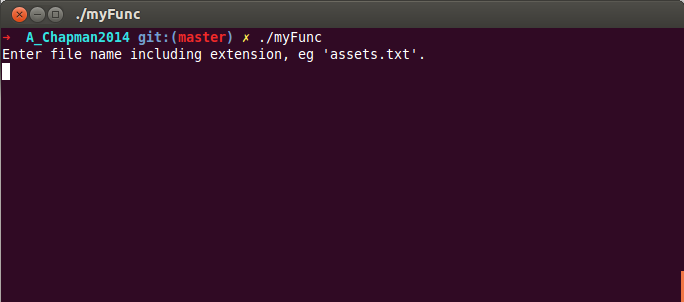
\includegraphics[width=0.9\textwidth]{asset_file}
  \caption{Enter file.}
  \label{fig:asset_file}
\end{figure}
After entering the correct name of the file, you will be asked to type in the number of particles for the swarm in PSO, no more than 50 is needed. Figure~\ref{fig:np} shows what you should see. 
\begin{figure}[H]
  \centering
    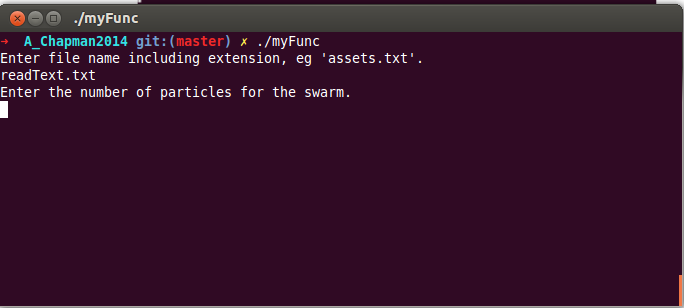
\includegraphics[width=0.9\textwidth]{np}
  \caption{Enter the number of particles}
  \label{fig:np}
\end{figure}
Then you will be asked to enter the number of iterations for the PSO to run for. Figure~\ref{fig:nit} shows what you should see. 
\begin{figure}[H]
  \centering
    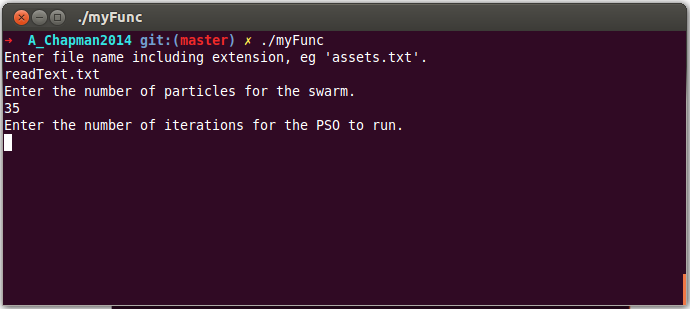
\includegraphics[width=0.9\textwidth]{nit}
  \caption{Enter number of iterations}
  \label{fig:nit}
\end{figure}
Followed the level of risk, 0.5 is neutral. Figure~\ref{fig:risk} shows what you should see. 
\begin{figure}[H]
  \centering
    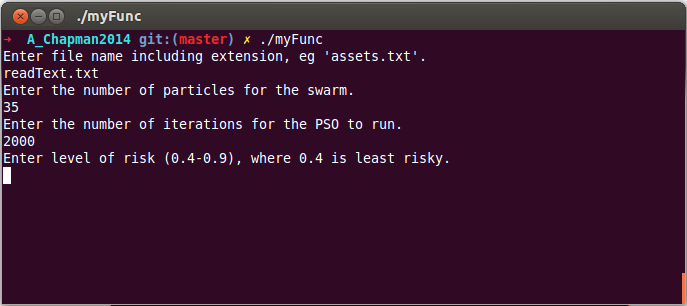
\includegraphics[width=0.9\textwidth]{risk}
  \caption{Enter level of risk}
  \label{fig:risk}
\end{figure}
Then input the lever of risk aversion, recommended is 3. Figure~\ref{fig:aversion} shows what you should see. 
\begin{figure}[H]
  \centering
    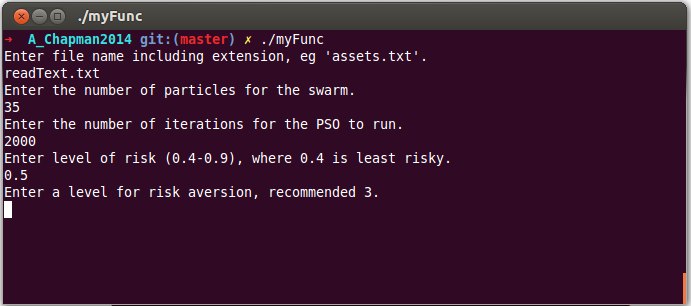
\includegraphics[width=0.9\textwidth]{aversion}
  \caption{Enter level of risk aversion}
  \label{fig:aversion}
\end{figure}
Finally, your expected required portfolio return. Figure~\ref{fig:portReq} shows what you should see. 
\begin{figure}[H]
  \centering
    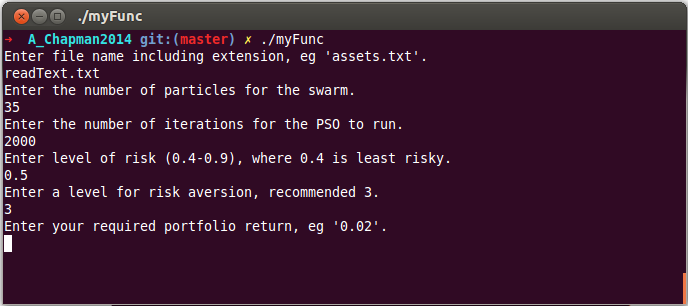
\includegraphics[width=0.9\textwidth]{portReq}
  \caption{Enter expected required return}
  \label{fig:portReq}
\end{figure} 
PSO is pretty quick so you will, if nothing was wrongly inputted, get an answer almost instantaneously. The system will display the ``un-prettified''results on the window. Figure~\ref{fig:results} shows what you should see. 
\begin{figure}[H]
  \centering
    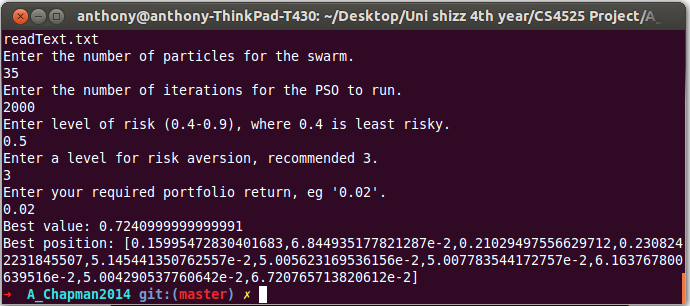
\includegraphics[width=0.9\textwidth]{results}
  \caption{Displaying results on command line}
  \label{fig:results}
\end{figure}
For the better looking results, open the folder containing the output file. The name will be ``output-(date).txt'' for example, output-(2014,5,1).txt. It will contain a file with the proportions of the optimal portfolio. Figure~\ref{fig:output} shows what you should see, where it states that you should invest 11.37\% on asset \textit{Aa}, 5.35\% on asset \textit{Bb}, and so on. 
\begin{figure}[H]
  \centering
    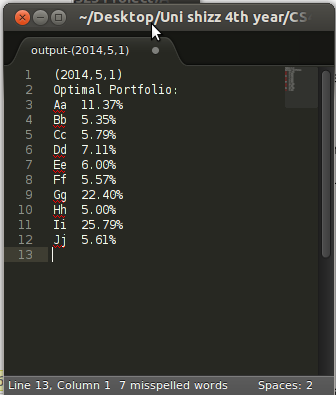
\includegraphics[width=0.9\textwidth]{output}
  \caption{Example output file.}
  \label{fig:output}
\end{figure}

\chapter*{Appendix B: Maintenance Manual}
The source code of the PSO and portfolio optimisation (together with an example asset file) could be found in the `source' folder in project submission.

\section*{Instructions on how to compile and run the algorithm:} 
  Makes sure that the source Haskell files (portOpt.hs, PSO.hs) are located in the same folder as the asset data files you wish to use for the portfolio.

  \begin{enumerate}
    \item Open a terminal and move to the folder containing the source files, ie the Haskell code.
    \item Type the following command into the terminal and press enter:
  \suspend{enumerate}
  \begin{center} \% ghc -O2 --make portOpt.hs -threaded -rtsopts \end{center}
  \resume{enumerate}
    \item You have now created an executable file, now type into the terminal the following and press enter:
  \suspend{enumerate}
  \begin{center} \% ./portOpt \end{center}
  \resume{enumerate}
    \item The program will start in the same terminal window.
  \end{enumerate}
  The User Manual provides a guide for using the program. \\

\section*{Organisation of System Files, including directory structures} 

\section*{Space and Memory Requirements}
  2 GB of RAM, 100 MB of space would be recommended.

\section*{List of source code files, with a summary of their role}
  \begin{tabular}{|l|l|}
    \hline
    File & Description \\
    \hline
    portOpt.hs & Portfolio optimisation implementation using PSO \\
    \hline
    PSO.hs & Main PSO optimisation module \\
    \hline
  \end{tabular}

\section*{Program Flow} 
  This section provides a general description of the program flow from a technical side. \\
  \textbf{Initialisation} \\

  \textbf{Optimisation} \\
  
  \textbf{Output} \\


\section*{Changing Parameters} 


\end{document}
